\section{پیاده‌سازی عملی}
به منظور تست الگوریتمی که در بخش پیشین ارائه گردید، یک ساختار نرم‌افزاری (فریم‌ورک) با نام \lr{Kompute} در زبان \lr{Kotlin} تعبیه شده است که مخزن آن در لینک زیر در دسترس می‌باشد:
\begin{latin}
	\begin{itemize}
		\item \href{https://github.com/dalisyron/Kompute}{https://github.com/dalisyron/Kompute}
	\end{itemize}
\end{latin}
با استفاده از این فریم‌ورک می‌توان الگوریتم جستجوی استراتژی تخلیه بهینه را به ازای پارامترهای محیطی مختلف اجرا کرد و عملکرد استراتژی بدست آمده از الگوریتم را با کمک شبیه‌سازی با سایر استراتژی‌ها مقایسه کرد. این فریم‌ورک طبق یافته‌های ما اولین پیاده‌سازی متن‌باز در زمینه استراتژی تخلیه وظایف ناهمگون است. \\

معماری کلی این فریم‌ورک در قالب یک کلاس دیاگرام در صفحه بعد آورده شده است.
\newpage
\begin{figure}[H]
	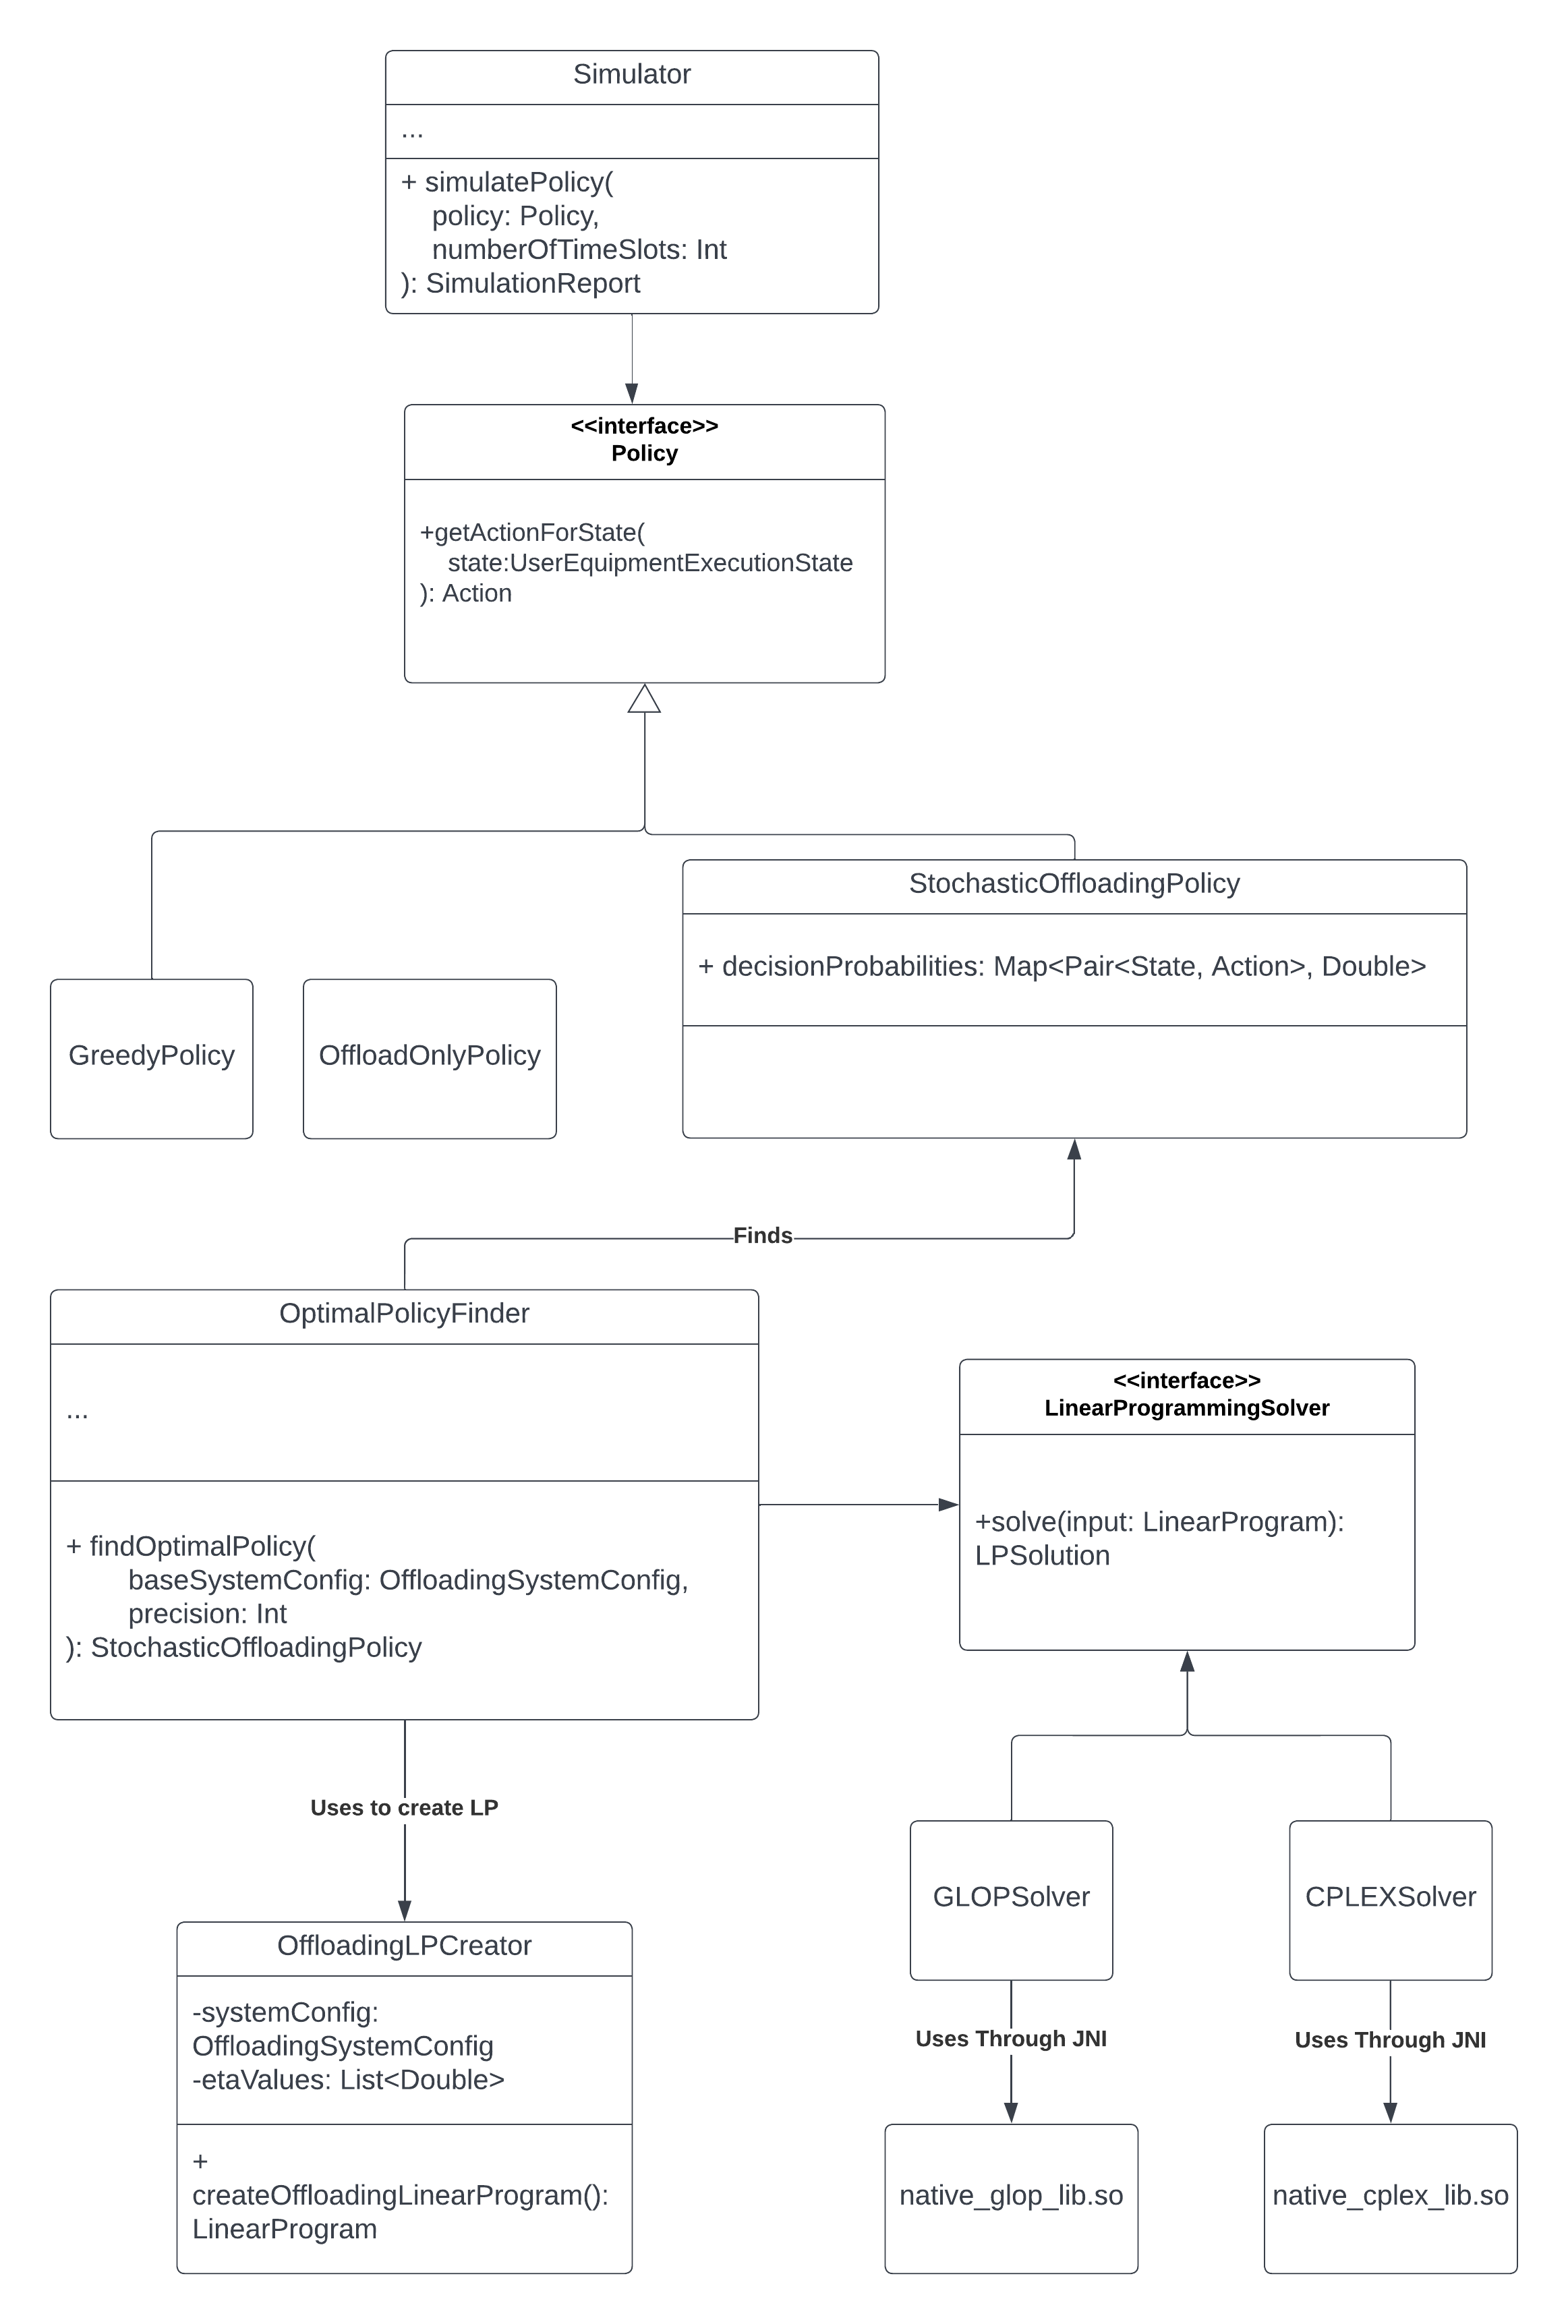
\includegraphics[width=0.9\textwidth]{cdiagram.png}
	\caption{کلاس دیاگرام فریم‌ورک \lr{Kompute}}
\end{figure}
\newpage
\subsection{ساخت و حل یک مسئله تخلیه وظیفه نمونه در \lr{Kompute}}
در کد نمونه زیر مسئله تخلیه وظیفه‌ برای محیط رایانش لبه‌ای با دو صف\footnote{شرایط بر اساس تقسیم‌بندی وظایف به \lr{Heavy} و \lr{Light} در اینترنت اشیا} حل شده است.
\begin{latin}
	\begin{lstlisting}[language=Kotlin]
		fun main(args: Array<String>) {
			val systemConfig = OffloadingSystemConfig(
			userEquipmentConfig = UserEquipmentConfig(
			stateConfig = UserEquipmentStateConfig(
			taskQueueCapacity = 5,
			tuNumberOfPackets = listOf(1, 3),
			cpuNumberOfSections = listOf(7, 2),
			numberOfQueues = 2
			),
			componentsConfig = UserEquipmentComponentsConfig(
			alpha = listOf(0.4, 0.9),
			beta = 0.90,
			etaConfig = null,
			pTx = 1.0,
			pLocal = 0.8,
			pMax = 1.7
			)
			),
			environmentParameters = EnvironmentParameters(
			nCloud = listOf(1, 1),
			tRx = 0.5,
			)
			)
			
			val optimalPolicy = RangedOptimalPolicyFinder.findOptimalPolicy(
			baseSystemConfig = systemConfig, 
			precision = 10
			)
			/*
			// For multi-threaded execution use this instead:
			
			val optimalPolicy = ConcurrentRangedOptimalPolicyFinder(
			baseSystemConfig = systemConfig
			).findOptimalPolicy(precision = 10, numberOfThreads = 8)
			*/
			
			
			val decisionProbabilities: Map<StateAction, Double>
			= optimalPolicy.stochasticPolicyConfig.decisionProbabilities
			
			println(decisionProbabilities)
		}
	\end{lstlisting}
\end{latin}
\newpage